\begin{frame}
\end{frame}

\begin{frame}
	\myheading{Module 21.1: Revisiting Autoencoders}
\end{frame}


\begin{frame}
	\begin{columns}
		\column{0.4\textwidth}
		\begin{overlayarea}{\textwidth}{\textheight}
			% LHS: figure of Autoencoder with the encoder decoder equations
			\vspace{3pt}
			\tikzstyle{input_neuron}=[circle,draw=red!50,fill=red!10,thick,minimum size=6mm]
\tikzstyle{hidden_neuron}=[circle,draw=blue!50,fill=cyan!10,thick,minimum size=6mm]
\tikzstyle{output_neuron}=[circle,draw=green!50,fill=green!10,thick,minimum size=6mm]

\tikzstyle{input}=[circle,draw=black!50,fill=black!20,thick,minimum size=6mm]

\begin{center}
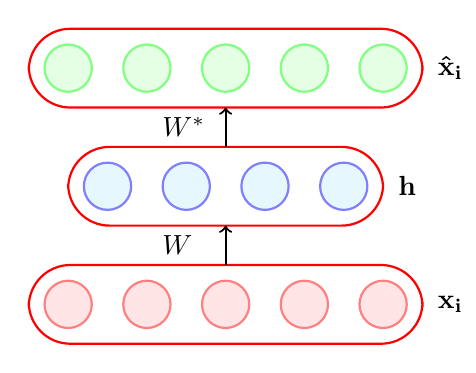
\begin{tikzpicture}

\node [input_neuron] (neuron01) at (6.5,4.5) {};
\node [input_neuron] (neuron02) at (7.5,4.5){};
\node [input_neuron] (neuron03) at (8.5,4.5) {};
\node [input_neuron] (neuron04) at (9.5,4.5) {};
\node [input_neuron] (neuron05) at (10.5,4.5) {};
\node [hidden_neuron] (neuron51) at (7,6) {} ;
\node [hidden_neuron] (neuron52) at (8,6)  {};
\node [hidden_neuron] (neuron53) at (9,6)  {};
\node [hidden_neuron] (neuron54) at (10,6)  {};

\node [output_neuron] (neuron11) at (6.5,7.5)  {};
\node [output_neuron] (neuron12) at (7.5,7.5)  {};
\node [output_neuron] (neuron13) at (8.5,7.5)  {};
\node [output_neuron] (neuron14) at (9.5,7.5)  {};
\node [output_neuron] (neuron15) at (10.5,7.5)  {};

\node[text width=0.01cm] at (11.2,4.5) {$\mathbf{x_i}$};
\node[text width=0.007cm] at (7.7,5.25) {$W$};
\node[text width=0.01cm] at (10.7,6) {$\mathbf{h}$};
\node[text width=0.007cm] at (7.7,6.75) {$W^*$};
\node[text width=0.01cm] at (11.2,7.5) {$\mathbf{\hat{x}_i}$};

\draw[red!100,thick,solid,rounded corners=15pt] (6,4) rectangle (11,5);
\draw[red!100,thick,solid,rounded corners=15pt] (6.5,5.5) rectangle (10.5,6.5);
\draw[red!100,thick,solid,rounded corners=15pt] (6,7) rectangle (11,8);



\draw[thick,->] (8.5,5) -- (8.5,5.5);

\draw[thick,->] (8.5,6.5) -- (8.5,7);



\end{tikzpicture}
\end{center}

			\vspace{-20pt}
			\begin{align*}
				\mathbf{h} &= g(W\mathbf{X} +\mathbf{b})\\
				\mathbf{\hat{X}} &= f(W^*\mathbf{h} +\mathbf{c})      
			\end{align*}

		\end{overlayarea}
		\column{0.6\textwidth}
		\begin{overlayarea}{\textwidth}{\textheight}
			\begin{itemize}[<+->]\justifying
				\item Before we start talking about VAEs, let us quickly revisit autoencoders
				\item An autoencoder contains an encoder which takes the input X and maps it to a hidden representation
				\item The decoder then takes this hidden representation and tries to reconstruct the input from it as $\hat{X}$
				\item The training happens using the following objective function
				\vspace{-0.1in}
				\small {
					\begin{align*} 
					& \min \limits_{W,W^*,\mathbf{c},\mathbf{b}}\hspace{0.5mm} \frac{1}{m}\sum_{i=1}^{m}\sum_{j=1}^{n} (\hat{x}_{ij}- x_{ij})^2 
					\end{align*}
				}
                \vspace{-0.1in}
                \item where $m$ is the number of training instances, $\{x_i\}_{i=1}^{m}$ and each $x_i \in R^n$ ($x_{ij}$ is thus the $j$-th dimension of the $i$-th training instance)
			\end{itemize}
		\end{overlayarea}
	\end{columns}
\end{frame}


\begin{frame}
	\begin{columns}
		\column{0.4\textwidth}
		\begin{overlayarea}{\textwidth}{\textheight}
			% LHS: same a previous slide
			\vspace{3pt}
			\tikzstyle{input_neuron}=[circle,draw=red!50,fill=red!10,thick,minimum size=6mm]
\tikzstyle{hidden_neuron}=[circle,draw=blue!50,fill=cyan!10,thick,minimum size=6mm]
\tikzstyle{output_neuron}=[circle,draw=green!50,fill=green!10,thick,minimum size=6mm]

\tikzstyle{input}=[circle,draw=black!50,fill=black!20,thick,minimum size=6mm]

\begin{center}
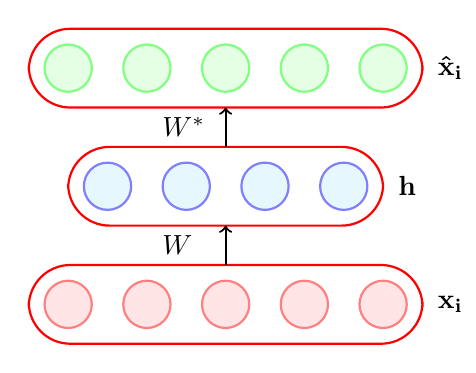
\begin{tikzpicture}

\node [input_neuron] (neuron01) at (6.5,4.5) {};
\node [input_neuron] (neuron02) at (7.5,4.5){};
\node [input_neuron] (neuron03) at (8.5,4.5) {};
\node [input_neuron] (neuron04) at (9.5,4.5) {};
\node [input_neuron] (neuron05) at (10.5,4.5) {};
\node [hidden_neuron] (neuron51) at (7,6) {} ;
\node [hidden_neuron] (neuron52) at (8,6)  {};
\node [hidden_neuron] (neuron53) at (9,6)  {};
\node [hidden_neuron] (neuron54) at (10,6)  {};

\node [output_neuron] (neuron11) at (6.5,7.5)  {};
\node [output_neuron] (neuron12) at (7.5,7.5)  {};
\node [output_neuron] (neuron13) at (8.5,7.5)  {};
\node [output_neuron] (neuron14) at (9.5,7.5)  {};
\node [output_neuron] (neuron15) at (10.5,7.5)  {};

\node[text width=0.01cm] at (11.2,4.5) {$\mathbf{x_i}$};
\node[text width=0.007cm] at (7.7,5.25) {$W$};
\node[text width=0.01cm] at (10.7,6) {$\mathbf{h}$};
\node[text width=0.007cm] at (7.7,6.75) {$W^*$};
\node[text width=0.01cm] at (11.2,7.5) {$\mathbf{\hat{x}_i}$};

\draw[red!100,thick,solid,rounded corners=15pt] (6,4) rectangle (11,5);
\draw[red!100,thick,solid,rounded corners=15pt] (6.5,5.5) rectangle (10.5,6.5);
\draw[red!100,thick,solid,rounded corners=15pt] (6,7) rectangle (11,8);



\draw[thick,->] (8.5,5) -- (8.5,5.5);

\draw[thick,->] (8.5,6.5) -- (8.5,7);



\end{tikzpicture}
\end{center}

			\vspace{-20pt}
			\begin{align*}
				\mathbf{h} &= g(W\mathbf{X} +\mathbf{b})\\
				\mathbf{\hat{X}} &= f(W^*\mathbf{h} +\mathbf{c})       
			\end{align*}
		\end{overlayarea}
		\column{0.6\textwidth}
		\begin{overlayarea}{\textwidth}{\textheight}
			\begin{itemize}\justifying
				\item<1-> But where's the fun in this ?
				\item<2-> We are taking an input and simply reconstructing it
				\item<3-> Of course, the fun lies in the fact that we are getting a good \textit{abstraction} of the input 
				\item<4-> But RBMs were able to do something more besides abstraction \onslide<5->{(they were able to do \textit{generation})}
				\item<6-> Let us revisit \textit{generation} in the context of autoencoders
			\end{itemize}
		\end{overlayarea}
	\end{columns}
\end{frame}


\begin{frame}
	\begin{columns}
		\column{0.4\textwidth}
		\begin{overlayarea}{\textwidth}{\textheight}
			% LHS: first same as previous slide, then on bullet 2 remove the encoder (read bullet 2)
			\vspace{3pt}
			\tikzstyle{input_neuron}=[circle,draw=red!50,fill=red!10,thick,minimum size=6mm]
\tikzstyle{hidden_neuron}=[circle,draw=blue!50,fill=cyan!10,thick,minimum size=6mm]
\tikzstyle{output_neuron}=[circle,draw=green!50,fill=green!10,thick,minimum size=6mm]

\tikzstyle{input}=[circle,draw=black!50,fill=black!20,thick,minimum size=6mm]

\begin{center}
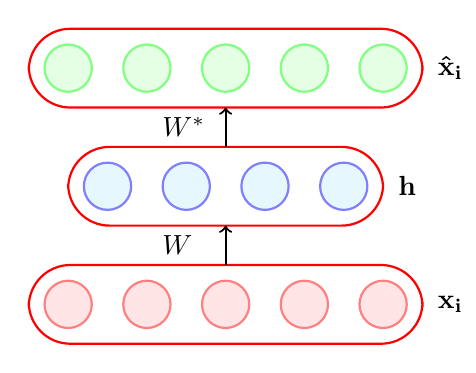
\begin{tikzpicture}

\onslide<1>{
\node [input_neuron] (neuron01) at (6.5,4.5) {};
\node [input_neuron] (neuron02) at (7.5,4.5){};
\node [input_neuron] (neuron03) at (8.5,4.5) {};
\node [input_neuron] (neuron04) at (9.5,4.5) {};
\node [input_neuron] (neuron05) at (10.5,4.5) {};
}
\node [hidden_neuron] (neuron51) at (7,6) {} ;
\node [hidden_neuron] (neuron52) at (8,6)  {};
\node [hidden_neuron] (neuron53) at (9,6)  {};
\node [hidden_neuron] (neuron54) at (10,6)  {};

\node [output_neuron] (neuron11) at (6.5,7.5)  {};
\node [output_neuron] (neuron12) at (7.5,7.5)  {};
\node [output_neuron] (neuron13) at (8.5,7.5)  {};
\node [output_neuron] (neuron14) at (9.5,7.5)  {};
\node [output_neuron] (neuron15) at (10.5,7.5)  {};

\onslide<1>{
\node[text width=0.01cm] at (11.2,4.5) {$\mathbf{x_i}$};
\node[text width=0.007cm] at (7.7,5.25) {$W$};
}
\node[text width=0.01cm] at (10.7,6) {$\mathbf{h}$};
\node[text width=0.007cm] at (7.7,6.75) {$W^*$};
\node[text width=0.01cm] at (11.2,7.5) {$\mathbf{\hat{x}_i}$};

\draw[red!100,thick,solid,rounded corners=15pt] (6,4) rectangle (11,5);
\draw[red!100,thick,solid,rounded corners=15pt] (6.5,5.5) rectangle (10.5,6.5);
\draw[red!100,thick,solid,rounded corners=15pt] (6,7) rectangle (11,8);



\draw[thick,->] (8.5,5) -- (8.5,5.5);

\draw[thick,->] (8.5,6.5) -- (8.5,7);



\end{tikzpicture}
\end{center}

			\vspace{-20pt}
%			\onslide<1->{\only<1>{\begin{align*}
%						\mathbf{h} &= g(W\mathbf{x_i} +\mathbf{b})
%			\end{align*}}}
			\begin{align*}
				\onslide<1>{\mathbf{h} &= g(W\mathbf{X} +\mathbf{b})\\}
				\mathbf{\hat{X}} &= f(W^*\mathbf{h} +\mathbf{c})    
			\end{align*}
		\end{overlayarea}
		\column{0.6\textwidth}
		\begin{overlayarea}{\textwidth}{\textheight}
			\begin{itemize}[<+->]\justifying
				\item Can we do generation with autoencoders ?
				\item In other words, once the autoencoder is trained can I remove the encoder, feed a hidden representation $h$ to the decoder and decode a $\hat{X}$ from it ?
				\item In principle, yes! But in practice there is a problem with this approach
				\item $h$ is a very high dimensional vector and only a few vectors in this space would actually correspond to meaningful latent representations of our input
				\item So of all the possible value of $h$ which values should I feed to the decoder (we had asked a similar question before: slide 67, bullet 5 of lecture 19)
			\end{itemize}
		\end{overlayarea}
	\end{columns}
\end{frame}


\begin{frame}
	\begin{columns}
		\column{0.4\textwidth}
		\begin{overlayarea}{\textwidth}{\textheight}
			% LHS: same as final figure from previous slide
			\vspace{3pt}
			\tikzstyle{input_neuron}=[circle,draw=red!50,fill=red!10,thick,minimum size=6mm]
\tikzstyle{hidden_neuron}=[circle,draw=blue!50,fill=cyan!10,thick,minimum size=6mm]
\tikzstyle{output_neuron}=[circle,draw=green!50,fill=green!10,thick,minimum size=6mm]

\tikzstyle{input}=[circle,draw=black!50,fill=black!20,thick,minimum size=6mm]

\begin{center}
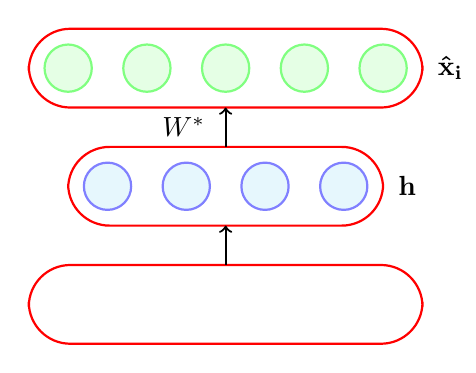
\begin{tikzpicture}

\node [hidden_neuron] (neuron51) at (7,6) {} ;
\node [hidden_neuron] (neuron52) at (8,6)  {};
\node [hidden_neuron] (neuron53) at (9,6)  {};
\node [hidden_neuron] (neuron54) at (10,6)  {};

\node [output_neuron] (neuron11) at (6.5,7.5)  {};
\node [output_neuron] (neuron12) at (7.5,7.5)  {};
\node [output_neuron] (neuron13) at (8.5,7.5)  {};
\node [output_neuron] (neuron14) at (9.5,7.5)  {};
\node [output_neuron] (neuron15) at (10.5,7.5)  {};

\node[text width=0.01cm] at (10.7,6) {$\mathbf{h}$};
\node[text width=0.007cm] at (7.7,6.75) {$W^*$};
\node[text width=0.01cm] at (11.2,7.5) {$\mathbf{\hat{x}_i}$};

\draw[red!100,thick,solid,rounded corners=15pt] (6,4) rectangle (11,5);
\draw[red!100,thick,solid,rounded corners=15pt] (6.5,5.5) rectangle (10.5,6.5);
\draw[red!100,thick,solid,rounded corners=15pt] (6,7) rectangle (11,8);



\draw[thick,->] (8.5,5) -- (8.5,5.5);

\draw[thick,->] (8.5,6.5) -- (8.5,7);



\end{tikzpicture}
\end{center}

			%\vspace{-20pt}
			\vspace{30pt}
			\begin{align*}
				\mathbf{\hat{X}} &= f(W^*\mathbf{h} +\mathbf{c})      
			\end{align*}
		\end{overlayarea}
		\column{0.6\textwidth}
		\begin{overlayarea}{\textwidth}{\textheight}
			\begin{itemize}\justifying
				\item<1-> Ideally, we should only feed those values of $h$ which are highly \textit{likely} 
				\item<2-> In other words, we are interested in sampling from $P(h|X)$ so that we pick only those $h$'s which have a high probability
				\item<3-> But unlike RBMs, autoencoders do not have such a probabilistic interpretation
				\item<4-> They learn a hidden representation $h$ but not a distribution $P(h|X)$
				\item<5-> Similarly the decoder is also deterministic and does not learn a distribution over $X$ (given a $h$ we can get a $X$ but not $P(X|h)$ )
			\end{itemize}
		\end{overlayarea}
	\end{columns}
\end{frame}

\begin{frame}
	\begin{block}{}
		We will now look at variational autoencoders which have the same structure as autoencoders but they learn a distribution over the hidden variables
	\end{block}
\end{frame}
